

\section{Vecindades}

Para poder observar cuantos pixeles vecinos debíamos tomar en cuenta para encontrar la dirección de la luz procedimos a hacer un breve experimento donde pintabamos de distintos colores los pixeles que consideraba mas brillante dependiendo la cantidad de vecindades. En este caso, donde mejor se pudo apreciar visualmente, se observa el punto negro con 0 vecindades (Solo él mismo), el punto rojo considera 2 pixeles vecinos, el punto verde son 4, el azul 6 vecindades, el amarillo 8 y el cian 10 pixeles vecinos.

\begin{figure}[h]
   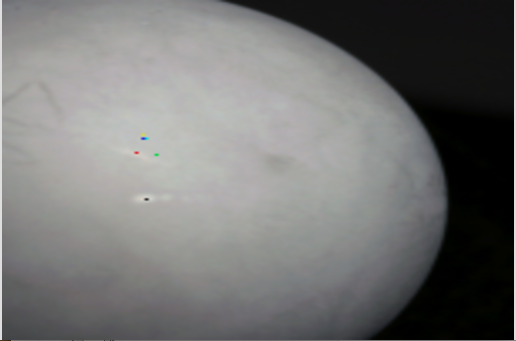
\includegraphics[scale=0.6]{ejemplo.png}
   \caption{Vecindades con ...}
   \label{Fig. 1}
\end{figure}

\indent La imágen se observan esos factores de los que hablamos en el desarrollo, entre aquellos, las manchas de distinto color y la aureola de luz. Pór ejemplo se ve el de vecindad 0 (púnto negro) bién lejos de los demas, por lo claro de la mancha blanca. Las vecindades de 2 y 4 (rojo y verde) también fueron corrompidos por el ruido, aunque llegaron un poco mas cerca. Luego a partir de los 6, 8 y 10 (azúl, amaríllo y cian) se podria creer que llega a un lugar en donde por más que agrandes el número de cantidad de vecindades no modificaria la posición, también viéndolo a simple vista se puede corroborar que es de dónde uno diria que proviene la luz.
\\
Prosiguiendo con las misma idea y utilizando las direcciones de luz obtenidas con vecindad 0 y vecindad 6,la cual consideramos la optima, obtuvimos distintos campos normales para la imágen del buda, observables a continuación:


\begin{figure}[h]
   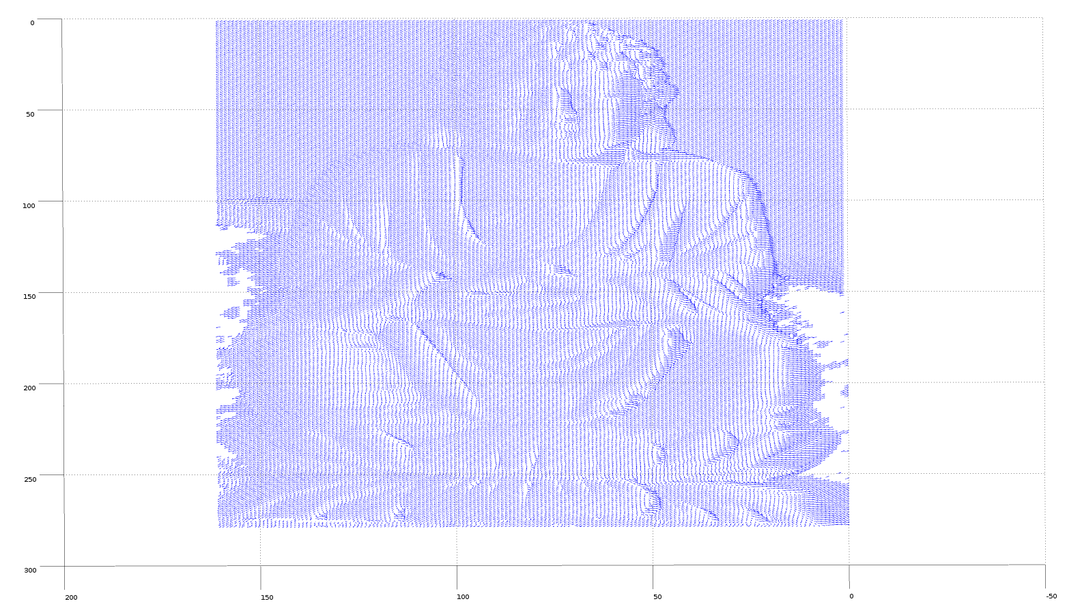
\includegraphics[scale=0.4]{buda_vecindad_0.png}
   \label{Fig. 2}
   \caption{Buda con vecindad 0}
\end{figure}

\begin{figure}[h]
   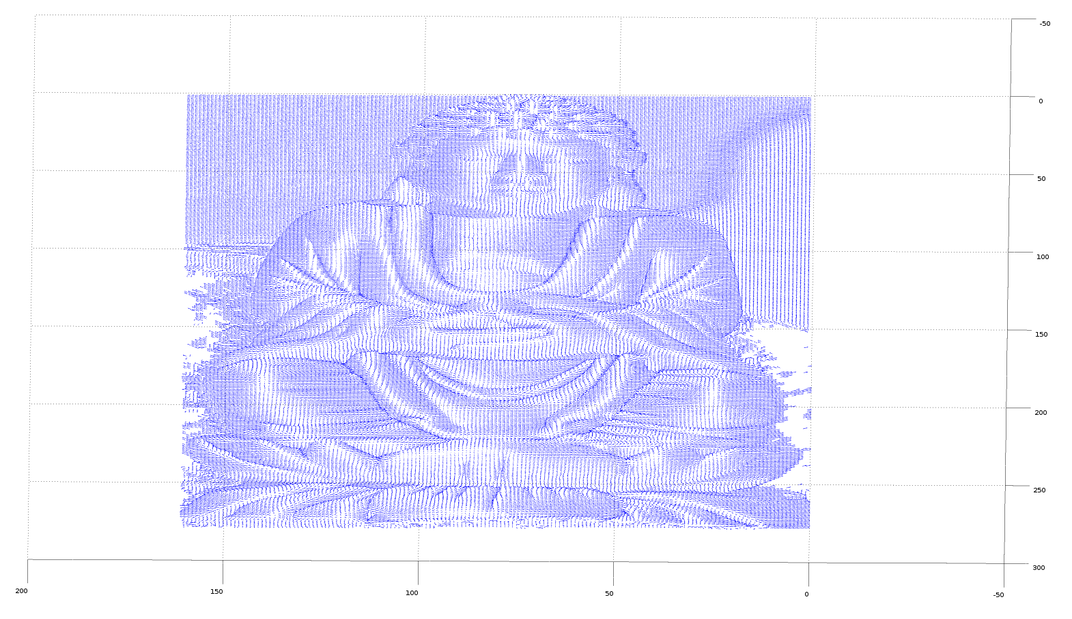
\includegraphics[scale=0.4]{buda_vecindades_6.png}
   \label{Fig. 3}
   \caption{Buda con vecindad 6}
\end{figure}



Concluimos con que modificar la cantidad de vecindades repercute fuertemente en la realización del resto del modelo, ya que con una mala dirección de la luz se perdera el efecto 3D, o mas bien parecera como que se obtuvo el efecto solo de uno de los lados (de derecha a izquierda). \par



\section{Número de condición}

La mejor forma de ver la diferencia entre dos matrices con distintos números de condición fue tomar la matrices con menor y con mayor número de condición asociados. De esta manera obtuvimos una matriz con un número de 15.0503 y otro con 407.581, una gran diferencia de tamaños. Luego para poder observar visualmente la dicerencia se le calculo el campo normal a cada uno, el resultado es el siguiente:



\begin{figure}[h]
   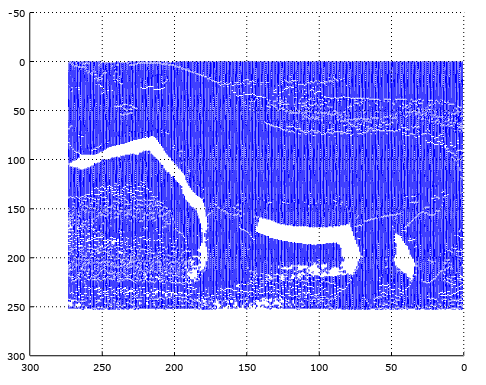
\includegraphics[scale=0.5]{caballoMax.png}
   \label{Fig. 4}
   \caption{Caballo con Número de condición de 407.581}
\end{figure}

\begin{figure}[h]
   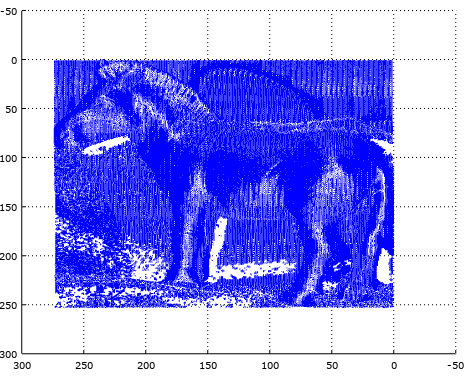
\includegraphics[scale=0.5]{caballoMin.png}
   \label{Fig. 5}
   \caption{Caballo con Número de condición de 15.0503}
\end{figure}


\section{Complejidades algoritmicas}

\indent Nuestra primer idea para tratar de comprobar nuestra hipótesis de que la factorización LU es mas rápida que la eliminación de gauss fue tomar distintos tamaños de matrices y triangularlos una vez con cada algoritmo para ver que método era mas rápido. Este experimento no pone a prueba nuestra hipótesis porque lo que intentábamos comprobar es que la factorización LU es mas rápida que la eliminación de gauss para resolver un sistema lineal despues de la primera vez que se resuelve el sistema. Si resolvíamos una sola vez cada tamaño de matriz, ambos algoritmos tardarían lo mismo. Por lo tanto, decidimos hacer un experimento donde mantuvimos constante el tamaño del sistema lineal a resolver y lo que variamos en cada instancia de testeo fueron las cantidades de términos independientes que debia resolver. Agregamos al mismo experimento la factorización de Cholesky.

\begin{figure}[h]
   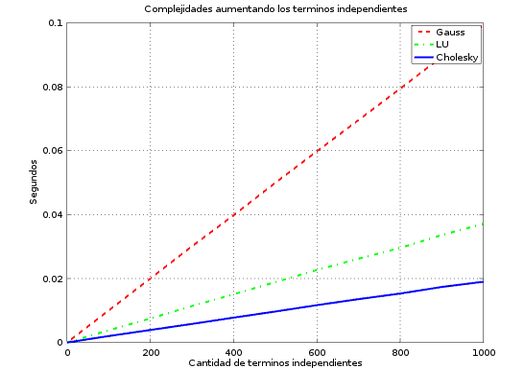
\includegraphics[scale=0.5]{ComplejidadesMalas.png}
   \label{Fig. 6}
   \caption{Resultado obtenido al aumentar la cantidad de terminos independientes}
\end{figure}

\indent Nuestra hipótesis, y a partir de lo que nos comentaron en las clases era que los algoritmos de eliminación gaussiana, factorización LU y Cholesky iban a tener un orden de complejidad cúbico y cuadrado, respectivamente, lo que al ver los resultados de las experimentaciones nos dice lo contrario. Las complejidades nos resultaron lineales.
Luego de consultarlo con la catedra, pudimos comprender que las complejidades no se iban a ver reflejadas en este experimento, ya que el tamaño de la matriz se mantenia igual. Por lo tanto debimos realizar un nuevo experimento en donde dejamos fijos en 100 terminos independientes a resolver y lo que se variaba en cada corrida era el tamaño de las matrices.


\begin{figure}[h]
   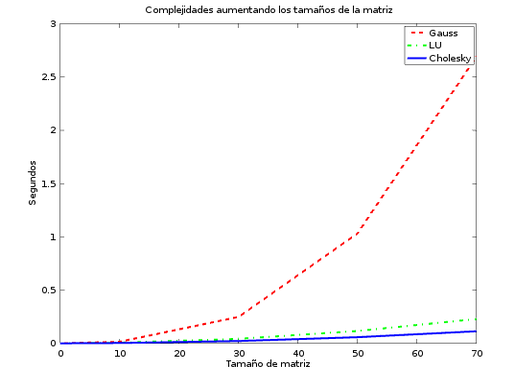
\includegraphics[scale=0.5]{complejidadesCorrecto.png}
   \label{Fig. 7}
   \caption{Resultado obtenido al aumentar la cantidad de terminos independientes}
\end{figure}